%!TEX root = ../../csuthesis_main.tex

\section{多无人机航迹规划及任务分配算法}

本节针对多无人机航迹规划及任务分配问题,构建了基于快速随机搜索树算法、A*算法、模拟退火算法、变邻域搜索算法的多无人机航迹规划及任务分配框架,该框架将多无人机航迹规划及任务分配问题划分为了无人机航迹规划阶段以及任务调度分配阶段,流程如图~\ref{fig:多无人机航迹规划及任务分配流程}所示,并针对这两个阶段,设计相应的算法。在无人机航迹规划阶段,提出了能够在静态场景下快速获得最优航迹的RRT*-Connect算法以及能够在动态场景下快速获得避障航迹的A*算法;在多无人机任务调度分配阶段,提出了基于模拟退火算法、变邻域算法以及温度自适应模拟退火算法\citep{wu2017SatelliteObservationSchedulinga}的变邻域结构搜索的温度自适应模拟退火算法(Temperature-adaptive Simulated Annealing Algorithm with Variable Neighborhood, TSAVN)。由RRT*-Connect生成无人机起飞点、任务点间的点与点的最优飞行航迹与航程,并利用生成的航程信息为TSAVN算法提供依据完成多无人机的任务调度。

\begin{figure}[!htbp]
    \centering
    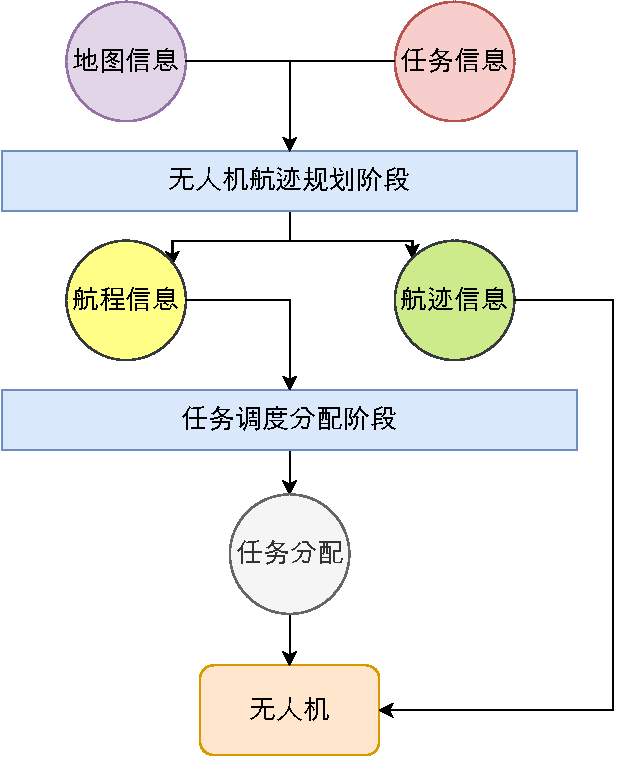
\includegraphics[width=0.5\textwidth]{images/多无人机任务分配及航迹规划流程.drawio.pdf}
    \caption{多无人机航迹规划及任务分配流程}
    \label{fig:多无人机航迹规划及任务分配流程}
\end{figure}

多无人机航迹规划及任务分配算法,是在无人机航迹规划及任务调度系统中由服务器为了解决无人机的配给及无人机航迹规划及任务分配问题所采用的算法,为了解决该问题,要求该算法能够在尽可能短的时间内确定最优的任务分配方案,包括

\begin{enumerate}[label=(\arabic*)]
    \item {所需无人机数目;}
    \item {各无人机所要执行的侦察任务有序序列;}
    \item {各无人机完成所给侦察任务有序序列的飞行航迹。}
\end{enumerate}

在服务器确定了以上内容后,会分配无人机并将对应的信息传输至无人机中,并由无人机自主根据所给指令完成所给侦察任务,在执行过程中,若出现了与飞行航迹冲突的障碍物,则再通过动态场景下的无人机航迹规划生成新的飞行航迹来规避障碍物。

\subsection{基于RRT*-Connect的静态场景下的无人机航迹规划算法设计}

静态场景下的无人机航迹规划算法,是用于在无人机执行任务前为无人机规划能够在尽可能短的时间内安全到达目标点执行任务的飞行航迹的措施。该算法根据已有的地图信息和任务信息,生成点间的最佳飞行航迹,以保障无人机飞行的安全性、稳定性,并确保能够快速到达任务地点执行任务。由于该算法是在任务执行前运行的,因此在可接受的运行时间下其生成的航迹规划结果的质量更为重要。

RRT算法是一种用于在高维非凸空间中通过构建路径树来生成路径的算法。这种树会通过随机在空间中采样来不断地拓展延伸,来探索未搜索的区域,最终达到目标点并得到起点至目标点的路径。\citet{lavalle1998RapidlyExploringRandomTrees}与\citet{lavalle2001RandomizedKinodynamicPlanninga}对RRT算法进行了延伸,使该算法能够解决存在着障碍物及不同约束的航迹规划问题中,也因此该算法被广泛运用在机器人的运动规划问题当中。

由于原始的RRT算法是完全在几何空间中随机采样,在运动规划问题当中会出现难以到达目标点,即难以收敛的现象,因此,为了改善这个问题,往往会在采样时让其有一定的概率选择目标点作为其采样点,并根据与目标点最近的树节点进行再取样,选取该树节点至目标点方向的不与障碍物相触碰的与该树节点间距不超过一定长度的新采样点作为新的树节点。

RRT-Connect算法是由\citet{kuffner2000RRTconnectEfficientApproachb}提出,在RRT算法的基础上,加入了Connect机制的新算法。Connect机制是在RRT的以起点为根节点的随机树的基础上,新增以目标点为根节点的随机树,在树的采样拓展过程中,两棵随机树交错着进行采样拓展,直至它们能够连接在一起,此时可以通过直接连接两棵树来得到从起点至目标点的路径。

RRT*算法则是用于解决RRT算法中存在的无法对路径进行优化的问题。该算法通过在路径采样拓展的过程中,采用了Rewire机制,通过对采样点与树节点的重布线,持续有效地对已有路径进行优化,使得在一定迭代次数和采样点的情况下,能够得到其中的最优且可行的路径。

\subsubsection{算法设计}

根据\citet{braun2019ComparisonRRTAlgorithmsa}的研究结果,由于RRT算法得到的路径是基于地图数据采样的结果,而非A*算法中基于启发式距离得到的路径,因此在精度高的地图中,使用RRT算法虽然得到的结果并不一定与A*算法得到的结果在质量上相当,但运算的速度会大幅提升。因此在无人机航迹规划算法的选择上,本文选择了以RRT算法为算法基础进行研究。

以上述所提及的算法为基础,本文采用了基于RRT*与RRT-Connect算法的RRT*-Connect算法,来完成无人机起飞点与任务点、任务点与任务点间的航迹规划及航程计算任务。

在RRT*-Connect算法中,给予所需的采样次数、选择随机采样的概率、地图信息、起点信息、目标点信息以及随机树单次拓展的最大长度,在每一次采样中,首先根据概率确定是选择从地图随机采样或是选择目标点,然后获取离随机树节点中离该采样点最近的树节点,随后根据给定的随机树单次拓展的最大长度进行重新采样,若点间长度符合长度约束则不需要重新采样,否则进行采样点进行调整,保证拓展的长度符合长度约束,然后再将采样点通过拓展的方式放入随机树中并对随机树使用Rewire机制进行路径优化,随后若该采样点能够放入另一棵随机树或已在另一棵随机树中,即两棵随机树能够进行连接,则将两颗树进行合并,此时即得到了最优解,然后在进入下一个循环前将两棵随机树的位置互换,确保两个树交错拓展,以上过程的伪代码如算法~\ref{alg:rrt*-connect}所示。

\begin{algorithm}[!htbp]
  \caption{RRT*-Connect算法} % 名称
  \label{alg:rrt*-connect}
  \begin{algorithmic}[1]
    \REQUIRE 
        \( n \):采样次数;
        \( p \):选择随机采样的概率;
        \( \mathcal{M} \):地图信息;
        \( \boldsymbol{x}_{\textrm{init}} \):起点信息;
        \( \boldsymbol{x}_{\textrm{goal}} \):目标点信息;
        \( \textrm{StepSize} \):随机树单次拓展的最大长度。
    \ENSURE 
        \( \Gamma \):从起点\( \boldsymbol{x}_{\textrm{init}} \)到目标点\( \boldsymbol{x}_{\textrm{goal}} \)的航迹;
        \( L \):从起点\( \boldsymbol{x}_{\textrm{init}} \)到目标点\( \boldsymbol{x}_{\textrm{goal}} \)的航迹的航程。
    \STATE 初始化随机树 \( \tau.\textrm{init}() \);
    \FOR{\( i = 1 \) to \( n \)}
        \IF{\( \textrm{Random()} \le p \)}
            \STATE \( \boldsymbol{x}_{\textrm{rand}} \gets \mathcal{M}.\textrm{sample}() \);
        \ELSE
            \STATE \( \boldsymbol{x}_{\textrm{rand}} \gets \boldsymbol{x}_{\textrm{goal}} \)
        \ENDIF
        \STATE \( \boldsymbol{x}_{\textrm{near}} \gets \textrm{Near}(\boldsymbol{x}_{\textrm{rand}}, \tau) \);
        \STATE \( \boldsymbol{x}_{\textrm{new}} \gets \textrm{Steer}(\boldsymbol{x}_{\textrm{rand}}, \boldsymbol{x}_{\textrm{near}}, \textrm{StepSize}) \);
        \IF{\( \textrm{Extend}(\tau, \boldsymbol{x}_{\textrm{new}}, \boldsymbol{x}_{\textrm{near}}) \ne \FALSE \)}
            \IF{\( \textrm{Connect}(\tau, \boldsymbol{x}_{\textrm{new}}) = \TRUE \)}
                \STATE \( \tau = \textrm{MergeTree}(\tau) \);
            \ENDIF
        \ENDIF
        \STATE \( \textrm{Swap}(\tau) \);
    \ENDFOR
    \STATE \( \Gamma \gets \tau.\textrm{getRoute}() \);
    \STATE \( L \gets \tau.\textrm{getRouteLength}() \);
  \end{algorithmic}
\end{algorithm}

在算法~\ref{alg:rrt*-connect}中,较为关键的部分为拓展函数,即Extend函数,该函数首先确定新的采样点在拓展进随机树后,新的航迹是否与障碍物发生碰撞,若发生碰撞则拓展失败;随后先获取一定数量的最近点,并寻找到能使树的根节点到该点的航程最小的树节点作为母节点进行拓展,如图~\ref{fig:寻找母节点进行拓展流程}所示,新拓展的节点为\( \boldsymbol{x}_{\textrm{new}} \),而以\( \boldsymbol{x}_{\textrm{init}} \)为根节点的随机树中,离该节点最近的\( \boldsymbol{x}_{\textrm{parent}} \)则为它默认的母节点,离该点稍远的\( \boldsymbol{x}_{\text{potential\_parent 1}} \)和\( \boldsymbol{x}_{\text{potential\_parent 2}} \)则为其潜在母节点,由于\( \boldsymbol{x}_{\textrm{potential\_parent 1}} \)至\( \boldsymbol{x}_{\textrm{new}} \)的线路上存在障碍物,故不考虑该点,而\( \boldsymbol{x}_{\textrm{potential\_parent 2}} \)与\( \boldsymbol{x}_{\textrm{new}} \)的路线上不会产生碰撞,且连接后从根节点\( \boldsymbol{x}_{\textrm{init}} \)到该节点的路径更短,因此将母节点修正为\( \boldsymbol{x}_{\textrm{potential\_parent 2}} \);

\begin{figure}[!htbp]
    \centering
    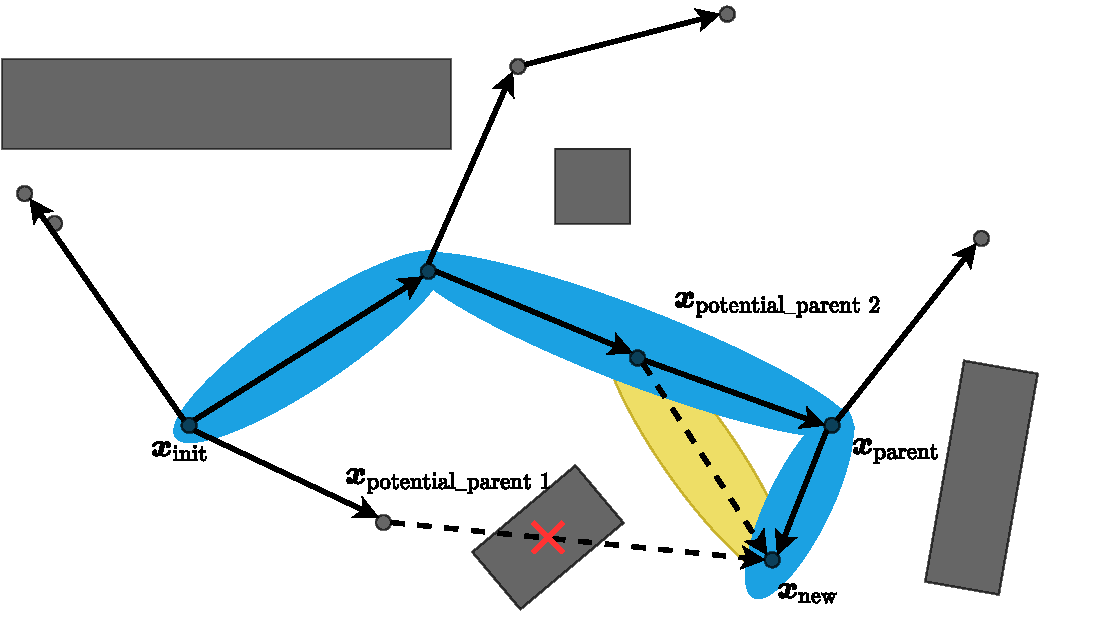
\includegraphics[width=0.8\textwidth]{images/choose_parent.pdf}
    \caption{寻找母节点进行拓展流程}
    \label{fig:寻找母节点进行拓展流程}
\end{figure}

在拓展完成后再以该点作为中间点,寻找是否存在一个树节点,使得根节点到新拓展的节点再到该树节点的航程,比根节点到该树节点的原本的航程要小,是则对该节点的连接方式进行调整,使起航迹的上一个节点为新拓展的节点,如图~\ref{fig:Rewire重布线流程}所示,在将采样点\( \boldsymbol{x}_{\textrm{new}} \)拓展入随机树后,存在着\( \boldsymbol{x}_{\textrm{potential\_child 1}} \)、\( \boldsymbol{x}_{\textrm{potential\_child 2}} \)以及\( \boldsymbol{x}_{\textrm{potential\_child 3}} \)三点潜在的子节点,但由于\( \boldsymbol{x}_{\textrm{init}} \to \boldsymbol{x}_{\textrm{new}} \to \boldsymbol{x}_{\textrm{potential\_child 1}} \)的航程大于\( \boldsymbol{x}_{\textrm{init}} \to \boldsymbol{x}_{\textrm{potential\_child 1}} \)的航程\( \boldsymbol{x}_{\textrm{init}} \to \boldsymbol{x}_{\textrm{new}} \to \boldsymbol{x}_{\textrm{potential\_child 3}} \)的航程大于\( \boldsymbol{x}_{\textrm{init}} \to \boldsymbol{x}_{\textrm{potential\_child 3}} \)的航程,\( \boldsymbol{x}_{\textrm{potential\_child 1}} \)和\( \boldsymbol{x}_{\textrm{potential\_child 3}} \)将不被考虑,而\( \boldsymbol{x}_{\textrm{init}} \to \boldsymbol{x}_{\textrm{new}} \to \boldsymbol{x}_{\textrm{potential\_child 2}} \)的航程小于\( \boldsymbol{x}_{\textrm{init}} \to \boldsymbol{x}_{\textrm{potential\_child 2}} \)的航程,故取消\( \boldsymbol{x}_{\textrm{potential\_child 2}} \)与\( \boldsymbol{x}_{\textrm{potential\_child 3}} \)的连接,新增\( \boldsymbol{x}_{\textrm{potential\_child 2}} \)与\( \boldsymbol{x}_{\textrm{new}} \)的连接,该机制为RRT-Connect算法的Rewire重布线机制。

\begin{figure}[!htbp]
    \centering
    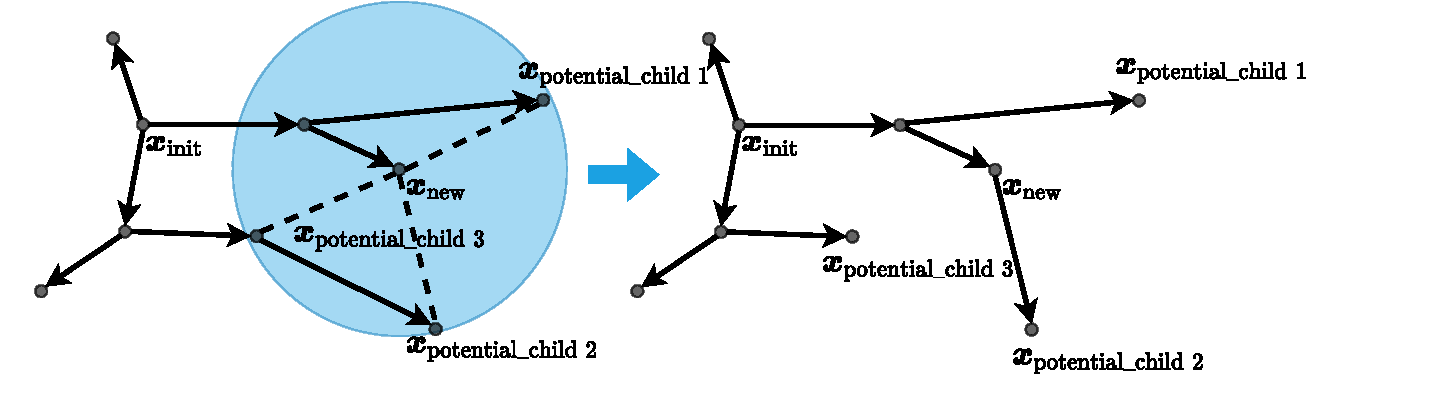
\includegraphics[width=\textwidth]{images/rewire.pdf}
    \caption{Rewire重布线流程}
    \label{fig:Rewire重布线流程}
\end{figure}

该函数的伪代码如算法~\ref{alg:extend_function}所示,为便于算法~\ref{alg:rrt*-connect}中判断采样点是否拓展入随机树成功,以便于接下来对随机树进行连接、合并等操作,故Extend函数需要将是否拓展如随机树成功的结果进行返回至上一层函数。

\begin{algorithm}[!htbp]
  \caption{Extend函数} % 名称
  \label{alg:extend_function}
  \begin{algorithmic}[1]
    \REQUIRE 
        \( \tau \):随机树;
        \( \boldsymbol{x}_{\textrm{new}} \):采样点;
        \( \boldsymbol{x}_{\textrm{near}} \):最近点。
    \ENSURE 
        \( S \):采样点拓展进随机树中是否成功。
    \IF{\( \textrm{CollisionFree}(\boldsymbol{x}_{\textrm{new}}) \)}
        \STATE \(\mathcal{X}_\textrm{near} \gets \textrm{NearC}(\tau, \boldsymbol{x}_{\textrm{new}}) \);
        \STATE \( \boldsymbol{x}_{\textrm{min}} \gets \textrm{ChooseParent}(\mathcal{X}_{\textrm{near}}, \boldsymbol{x}_{\textrm{near}}, \boldsymbol{x}_{\textrm{new}}) \);
        \STATE \( \tau.\textrm{addNodeEdge}(\boldsymbol{x}_{\textrm{min}}, \boldsymbol{x}_{\textrm{new}}) \);
        \STATE \( \tau.\textrm{rewire}() \);
        \RETURN \TRUE;
    \ENDIF
    \RETURN \FALSE;
  \end{algorithmic}
\end{algorithm}

\subsection{基于A*的动态场景下的无人机航迹规划算法设计}

动态场景下的无人机航迹规划算法,是用于为单体无人机提供应对可能存在突发事况的动态环境下的措施。该算法根据已有的地图信息和配备的传感器探测到的障碍物信息,对由服务器为其规划的路径进行修订,保障其飞行的安全性与稳定性,并确保能够及时到达任务地点。由于该算法是在无人机飞行过程中运行的,需要实时对飞行航迹进行修改,因此该算法对运行时间有着较高的要求。

\subsubsection{算法设计}

同样根据\citet{braun2019ComparisonRRTAlgorithmsa}的研究结果,在大小较大且精度较低或大小较小且精度较高的地图信息中寻找最短路径,使用A*及其派生算法得到的路径不论是从稳定性还是从运算速度上看,都远远好于RRT及其派生算法。而在单无人机的实时避障算法中,由于其对航迹修订的范围仅为无人机传感器能够感知的范围,属于精度较高但地图大小较小的类型,因此适用A*算法来解决该问题。

A*算法最初由\citet{hart1968FormalBasisHeuristica}提出,是将启发式的方法如BFS等,应用于常规的方法如Dijkstra算法等的一种算法。该算法通过逐步对每一个节点\( n \)进行从起点经过该点再至目标点的估计代价或距离,来不断更新优化,最终得到地图信息中从起点到目标点的最短路径,其距离的估计函数用公式表达为:

\begin{equation}
    f(n) = g(n) + h(n) \nonumber
\end{equation}

其中,\( f(n) \)为对于节点\( n \),从起点经过该点再至目标点的估计代价或距离;\( g(n) \)为从起点至节点\( n \)的实际距离;\( h(n) \)为从节点\( n \)至目标点的估计距离,通常用欧式距离,即\( d(\boldsymbol{x}_n, \boldsymbol{x}_0) = \parallel \boldsymbol{x}_n - \boldsymbol{x}_0 \parallel ^ 2\),进行估计。

A*算法的流程的伪代码如算法~\ref{alg:A-Star}所示。

\begin{algorithm}[!htbp]
  \caption{A*算法} % 名称
  \label{alg:A-Star}
  \begin{algorithmic}[1]
    \REQUIRE
      $M$: 地图信息;
      $S$: 起点信息;
      $D$: 目标点信息;
    \ENSURE
      $P$: 飞行航迹;
    \STATE 初始化集合 \( L \gets \text{init}(S)\);
    \WHILE {\( ! \text{L.isEmpty}() \)}
        \STATE 估计距离最小的节点 \( p_\textrm{min\_fn} \gets \textrm{FindMin}(L) \);
        \IF{\( p_\textrm{min\_fn} == D \)}
            \STATE \( P \gets \textrm{GetTrajectory}(p_{\textrm{min\_fn}}) \);
            \STATE break;
        \ENDIF
        \STATE 获取四周尚未搜索过的节点 \( p_\textrm{unexplored} \gets \text{FindNew} (p_{\textrm{min\_fn}}) \);
        \FORALL{\( p_{\textrm{cur}} \) in \(p_\textrm{unexplored}\)}
            \IF {\( \text{IsBlockedByEnv}(p_{\textrm{cur}}) \)}
                \STATE continue;
            \ENDIF
            \STATE 将可行节点添加入集合中 \( \text{L.add}(p_{\textrm{cur}})\);
        \ENDFOR
    \ENDWHILE
    \RETURN \( P \);
  \end{algorithmic}
\end{algorithm}

\subsubsection{算法应用流程}

以图~\ref{fig:单无人机避障实际场景示例}为例,假设实际场景中的障碍物如图~\ref{fig:单无人机避障实际场景示例}中的分布,此时无人机以到达图中的位置,继续沿着原定的飞行航迹前往目标点,而原本为该无人机规划的飞行航迹和已知的地图信息则如图~\ref{fig:单无人机避障规划示例}所示。很明显,已知的地图信息与实际信息存在可能在精细度上的差异,缺失了在飞行航迹中存在的障碍物,导致若无人机按照原本规划的飞行航迹不进行修订,则该无人机将会与障碍物发生碰撞从而造成无人机损毁及侦察任务的无法完成。

\begin{figure}[!htbp]
    \centering
    \begin{subfigure}[t]{0.48\textwidth}
        \captionsetup{justification=centering}
        \begin{minipage}[b]{\linewidth}
            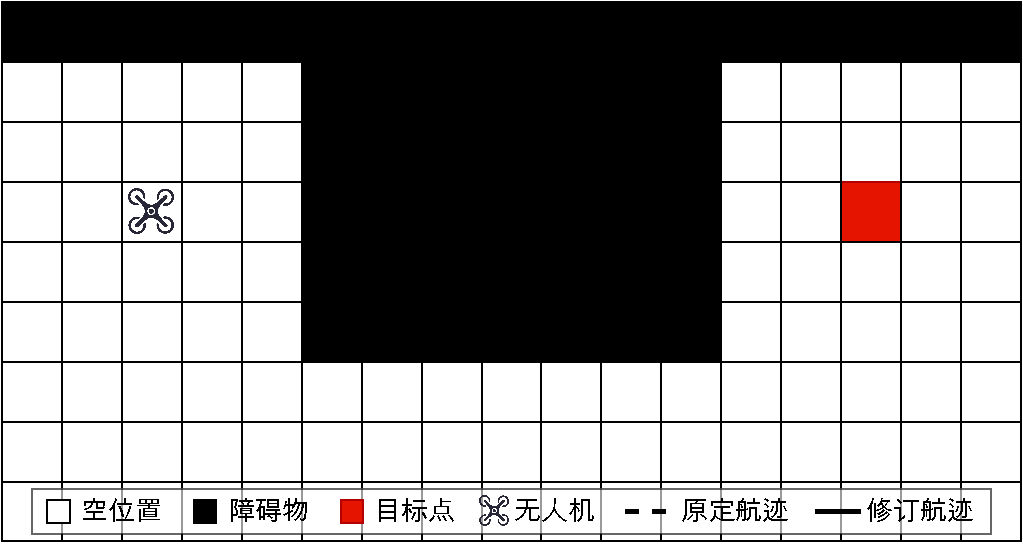
\includegraphics[width=\textwidth]{images/单无人机避障实际场景示例.pdf}
            \caption{单无人机避障实际场景示例}
            \label{fig:单无人机避障实际场景示例}
        \end{minipage}
    \end{subfigure}
    \begin{subfigure}[t]{0.48\textwidth}
        \captionsetup{justification=centering}
        \begin{minipage}[b]{\linewidth}
            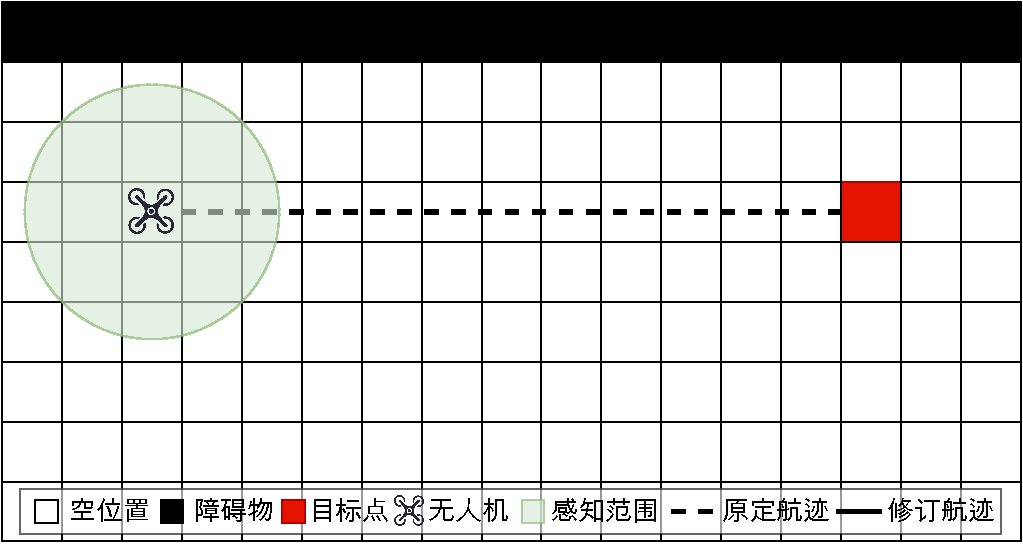
\includegraphics[width=\textwidth]{images/单无人机避障规划场景示例.pdf}
            \caption{单无人机避障规划示例}
            \label{fig:单无人机避障规划示例}
        \end{minipage}
    \end{subfigure}
    \caption{单无人机避障示例}
    \label{fig:单无人机避障示例}
\end{figure}

此时,该无人机可以根据其自身携带的能够探测障碍物的传感器设备,如成本高昂但精度与探测范围都很高的激光雷达、成本低廉但精度及探测范围较差的超声波探测器等,通过不断地对已有的地图信息进行修正,并运行A*算法来修订原有航迹,最终平安无事地到达任务点执行侦察任务。以图~\ref{fig:单无人机避障示例}中的情景为例,无人机在按照原有航迹进行飞行前行时,传感器探测到前方存在障碍物,此时运行A*算法进行航迹的修订,之后按照修订后的航迹进行飞行,如图~\ref{fig:单无人机第一次修订航迹进行避障}所示;但此时无人机所存储的地图信息明显与图~\ref{fig:单无人机避障实际场景示例}中不同,按新的航迹前行仍然会障碍物相撞,因此在无人机继续前行时,依然检测到了与航迹存在冲突的障碍物,此时需再运行A*算法,进一步修订飞行航迹,如图~\ref{fig:单无人机第二次修订航迹进行避障}所示;在完成对障碍物正面的绕行后,无人机继续检测到了与航迹冲突的障碍物,再一次运行了A*算法对航迹进行修订,如图~\ref{fig:单无人机第三次修订航迹进行避障}所示;不断重复以上过程,如图~\ref{fig:单无人机第四次修订航迹进行避障}、图~\ref{fig:单无人机第五次修订航迹进行避障}和图~\ref{fig:单无人机第六次修订航迹进行避障}所示,直至无人机能够顺利沿着修订航迹到达任务点的位置。

\begin{figure}[!htbp]
    \centering
    \begin{subfigure}[t]{0.48\textwidth}
        \captionsetup{justification=centering}
        \begin{minipage}[b]{\linewidth}
            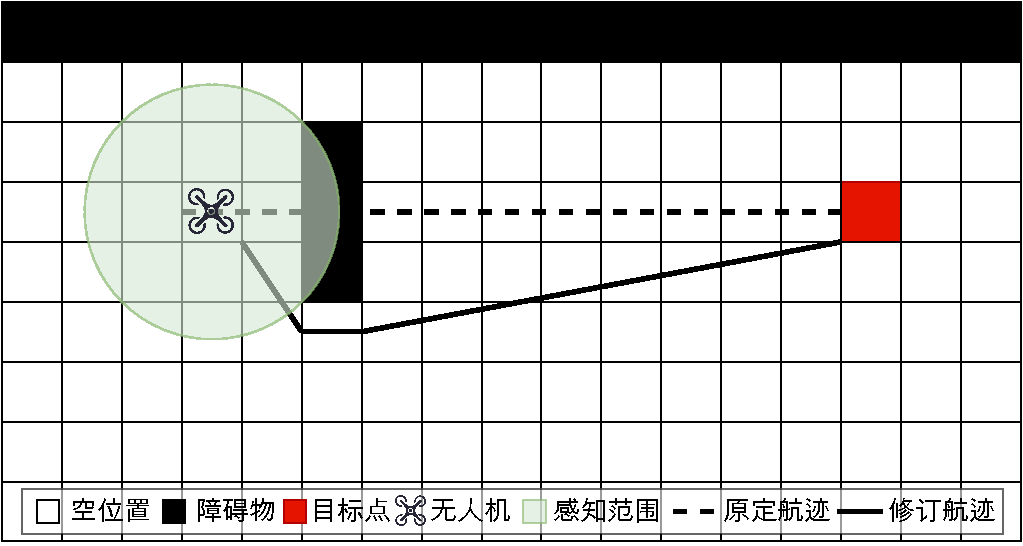
\includegraphics[width=\textwidth]{images/单无人机避障步骤示例1.pdf}
            \caption{无人机第一次修订航迹进行避障}
            \label{fig:单无人机第一次修订航迹进行避障}
        \end{minipage}
    \end{subfigure}
    \begin{subfigure}[t]{0.48\textwidth}
        \captionsetup{justification=centering}
        \begin{minipage}[b]{\linewidth}
            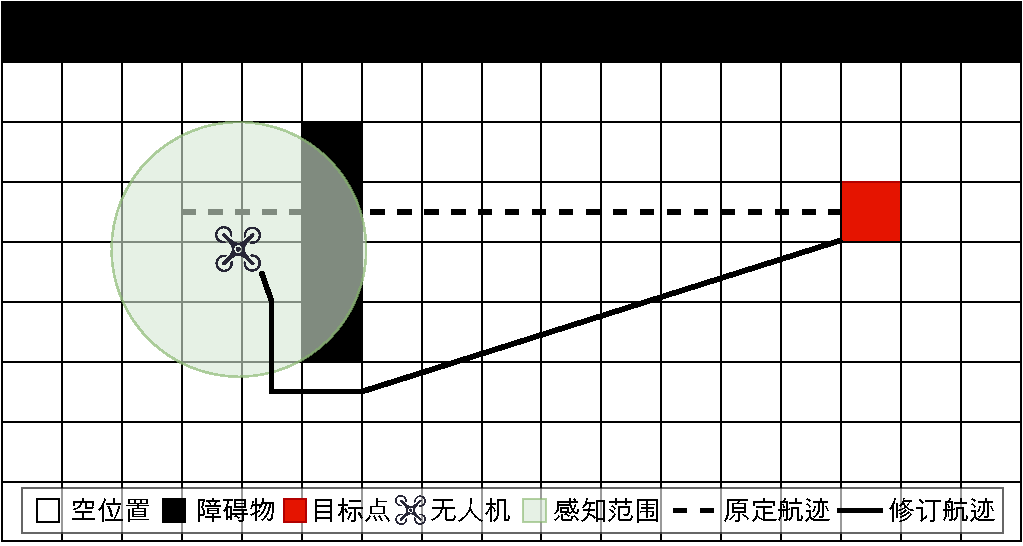
\includegraphics[width=\textwidth]{images/单无人机避障步骤示例2.pdf}
            \caption{无人机第二次修订航迹进行避障}
            \label{fig:单无人机第二次修订航迹进行避障}
        \end{minipage}
    \end{subfigure}
    \begin{subfigure}[t]{0.48\textwidth}
        \captionsetup{justification=centering}
        \begin{minipage}[b]{\linewidth}
            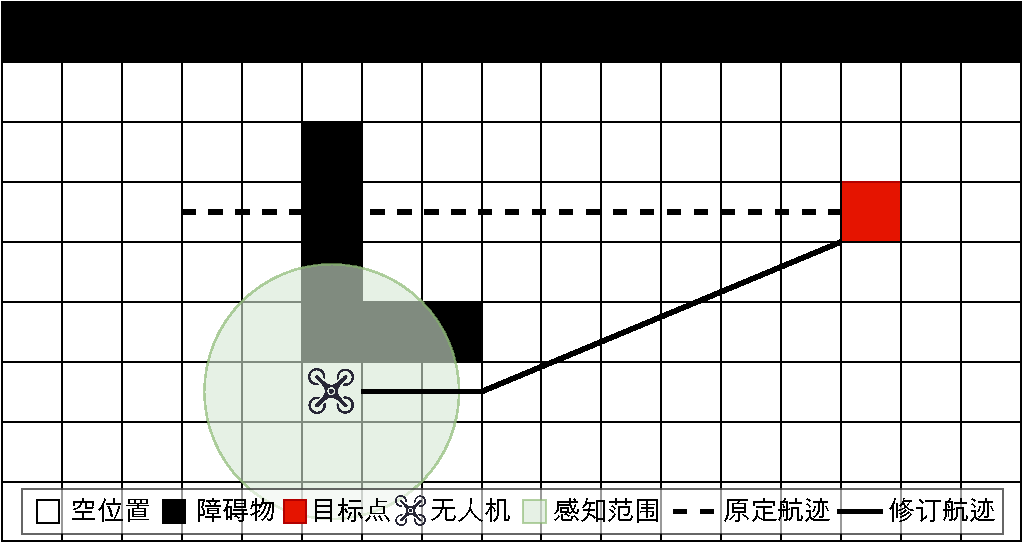
\includegraphics[width=\textwidth]{images/单无人机避障步骤示例3.pdf}
            \caption{无人机第三次修订航迹进行避障}
            \label{fig:单无人机第三次修订航迹进行避障}
        \end{minipage}
    \end{subfigure}
    \begin{subfigure}[t]{0.48\textwidth}
        \captionsetup{justification=centering}
        \begin{minipage}[b]{\linewidth}
            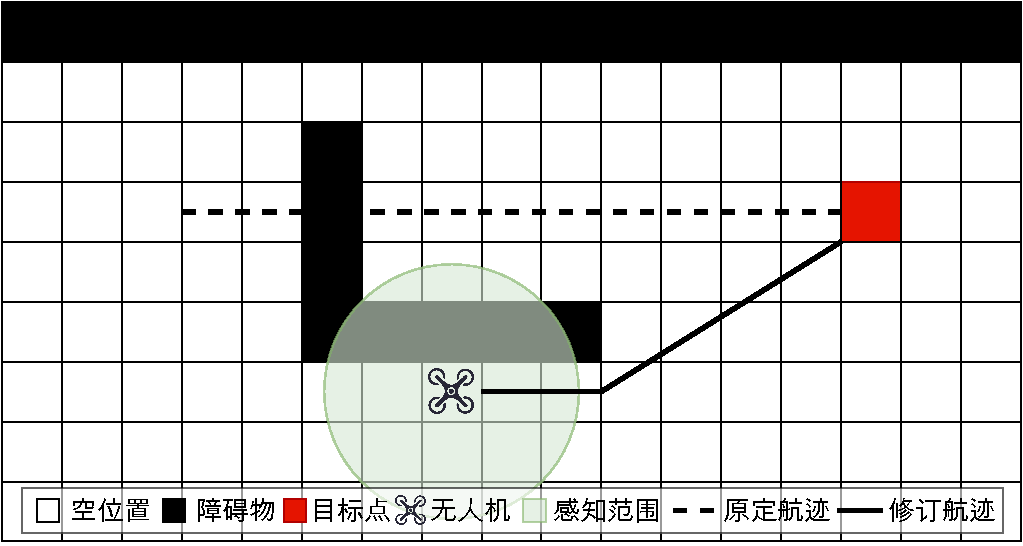
\includegraphics[width=\textwidth]{images/单无人机避障步骤示例4.pdf}
            \caption{无人机第四次修订航迹进行避障}
            \label{fig:单无人机第四次修订航迹进行避障}
        \end{minipage}
    \end{subfigure}
    \begin{subfigure}[t]{0.48\textwidth}
        \captionsetup{justification=centering}
        \begin{minipage}[b]{\linewidth}
            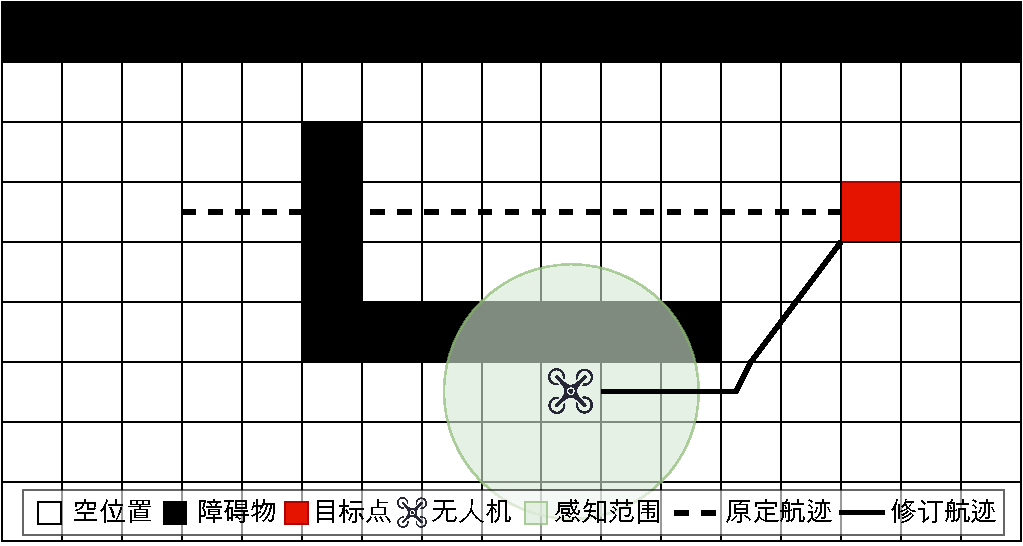
\includegraphics[width=\textwidth]{images/单无人机避障步骤示例5.pdf}
            \caption{无人机第五次修订航迹进行避障}
            \label{fig:单无人机第五次修订航迹进行避障}
        \end{minipage}
    \end{subfigure}
    \begin{subfigure}[t]{0.48\textwidth}
        \captionsetup{justification=centering}
        \begin{minipage}[b]{\linewidth}
            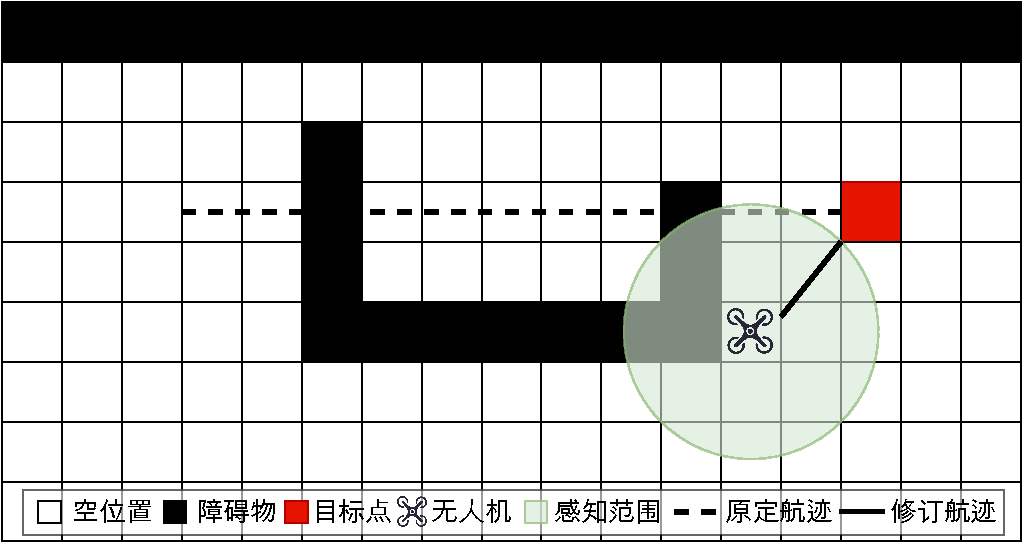
\includegraphics[width=\textwidth]{images/单无人机避障步骤示例6.pdf}
            \caption{无人机第六次修订航迹进行避障}
            \label{fig:单无人机第六次修订航迹进行避障}
        \end{minipage}
    \end{subfigure}
    \caption{无人机实时修订航迹进行避障}
    \label{fig:单无人机实时修订航迹进行避障}
\end{figure}

\subsubsection{算法流程图}

根据上述内容,本文提出的单无人机下的实时避障算法的运行流程如下,在无人机收到指令后或完成上一任务点的收集型侦察任务后,由无人机的飞行控制系统控制无人机按照所给飞行航迹进行飞行,并在飞行过程中不断地根据障碍物探测传感器的结果更新其地图数据库储存的地图信息,根据该地图信息来判断当前无人机的飞行航迹是否与已探测到的障碍物存在冲突,若存在冲突,则调用A*算法,先计算当前无人机与航迹点的估计距离,再更新周围点的估计距离,之后不断更新已知点中估计距离最小的点的周围点的估计距离,直到到达目标点,此时根据得到的修订航迹对原有飞行航迹进行修订,直到到达当前任务点开始执行收集型侦察任务。总流程如图~\ref{fig:单无人机避障算法流程图}所示。

\begin{figure}[!htbp]
    \centering
    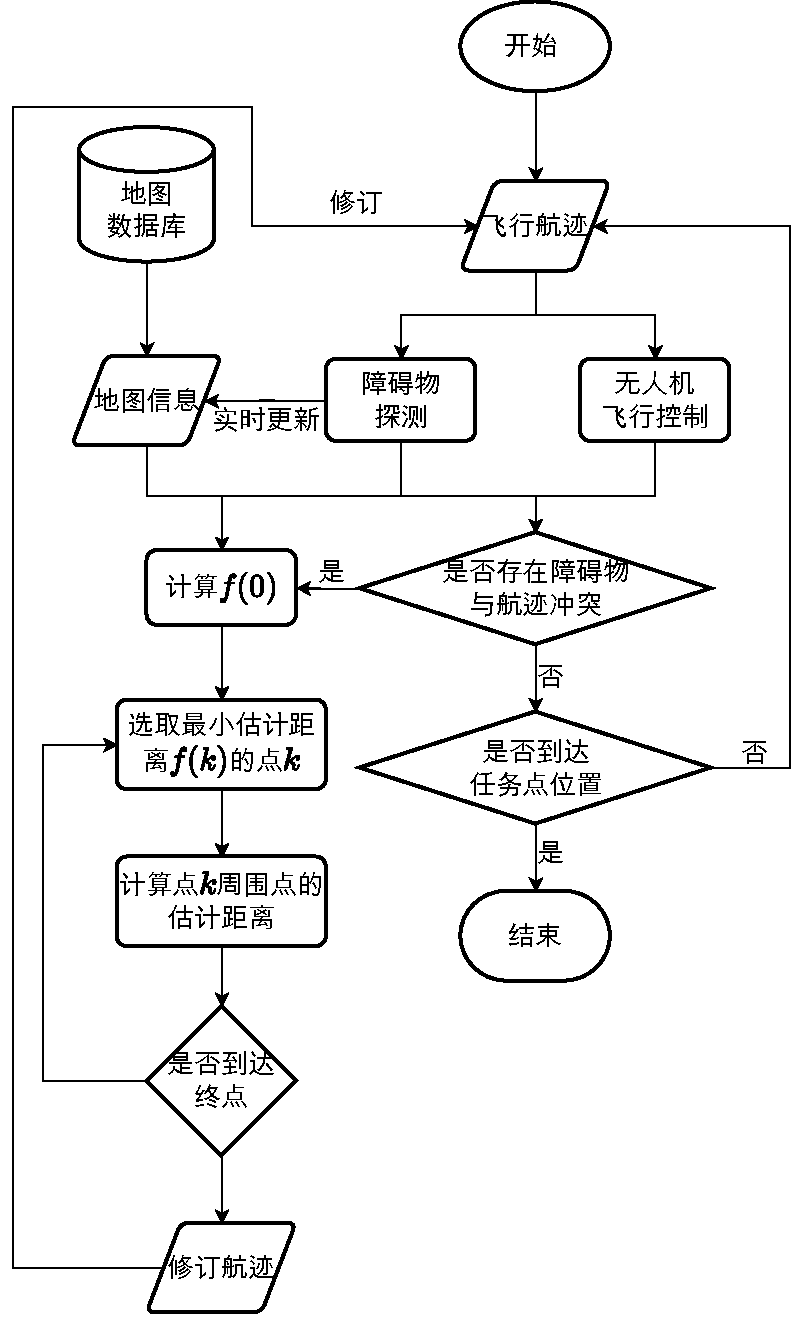
\includegraphics[width=0.7\textwidth]{images/单无人机避障算法总流程图.pdf}
    \caption{单无人机避障算法流程图}
    \label{fig:单无人机避障算法流程图}
\end{figure}
